\documentclass[11pt,a4paper]{article}
\usepackage{tikz}
\usetikzlibrary{arrows.meta,positioning}
\usepackage{tabularx}
\usepackage{amsmath,amssymb,amsthm}
\usepackage{geometry}
\geometry{margin=1in}
\usepackage{hyperref}
\usepackage{graphicx}
\usepackage{setspace}
\onehalfspacing

\title{\textbf{Paper F-01: Stellar Evolution:\\ A Constraint-Driven Flux Dynamics (CDFD) Perspective}}
\author{Steve Bico Mujjabi, MD\\
\small Independent Researcher\\
\small Founder, Vura Labs\\
\small Kampala, Uganda\\
\small ORCID: 0009-0001-0556-5516}
\date{May 2026}

\begin{document}
\maketitle


\begin{abstract}
This paper develops a falsifiable CDFD/AFL model of Stellar Evolution. It maps nuclear energy generation, radiative transport, and mass flow to driving flux $\Phi$, gravity, opacity, fuel availability, and transport limits to active constraint $C$, convection, expansion, fusion regulation, mass loss, and mixing to responsiveness $S$, and composition, rotation, magnetic state, and prior burning stages to structural memory $M_s$. The target outcome is luminosity, stability, nucleosynthesis, and evolutionary transition, tested against photometry, spectroscopy, asteroseismology, neutrinos, stellar populations, and models. The paper treats universality as a shared model architecture rather than an assertion that unlike systems have the same material mechanism. It states the negative result that would make the mapping unnecessary and places the domain claim inside the cumulative CDFD programme and its reproducible runtime boundary.
\end{abstract}

\section*{Symbol Conventions}

\noindent\textbf{CDFD/AFL Part IV symbol convention.}
\begin{center}
{\small
\begin{tabular}{p{0.15\linewidth}p{0.34\linewidth}p{0.41\linewidth}}
\hline
Symbol & Part IV meaning & Cross-domain reading \\
\hline
$\Phi$ & Driving flux or throughput & Energy, matter, signal, capital, information, traffic, force, or biological load entering a system \\
$C$ & Active constraint or capacity burden & Bottleneck, resistance, boundary, scarcity, toxicity, regulation, topology, latency, or load-bearing limit \\
$S$ & Responsiveness or adaptive surface & The system's ability to reconfigure, buffer, route, repair, learn, or preserve function under changing load \\
$M_s$ & Structural memory & Stored damage, hysteresis, inherited topology, institutional memory, trained weights, ecological legacy, or retained state \\
$\Psi_s$ & Adaptive operating ratio $(\Phi/C)\cdot S\cdot M_s$ & Local bookkeeping gauge for constrained operation, overload, recovery, or regime change; not a universal constant \\
$\Lambda$ & Life Number or capstone surplus ratio where explicitly defined & Reserved for Part II-derived life-number notation or synthesis-level surplus measures, never an undefined decoration \\
\hline
\end{tabular}
}
\end{center}

\noindent\textbf{Greek-symbol convention.}
\begin{center}
{\small
\begin{tabular}{p{0.15\linewidth}p{0.34\linewidth}p{0.41\linewidth}}
\hline
Symbol & Local role & Interpretation rule \\
\hline
$\alpha$ & Accumulation or reinforcement coefficient & Sets how fast a pathway, constraint, habit, cascade, or retained structure grows under load \\
$\beta$ & Relaxation, decay, clearance, or washout coefficient & Sets loss, recovery, damping, forgetting, degradation, or return toward baseline \\
$\gamma$ & Coupling, diffusion, redistribution, or transfer coefficient & Sets spread across nodes, layers, tissues, markets, infrastructures, media, or physical phases \\
$\delta,\epsilon$ & Perturbation, tolerance, small offset, or numerical guard & Used only as local thresholds, stability margins, measurement tolerances, or stress increments \\
$\eta,\lambda,\mu,\nu$ & Efficiency, rate, baseline, intensity, or frequency terms & Meaning is fixed by the equation, subscript, and domain-specific proxy in the paragraph where the term appears \\
$\rho,\sigma,\tau,\phi$ & Density/correlation, variability/noise, time-scale, phase, or field terms & Local coefficients only; subscripts bind them to the named pathway, domain, or experiment \\
$\Omega,\Lambda$ & Domain/state space; Life Number where defined & $\Omega$ names a modeled state space; $\Lambda$ carries life-number or synthesis notation only when the paper defines it \\
\hline
\end{tabular}
}
\end{center}

\section{Series Context}

Part I sets the flow--constraint language used here \cite{MujjabiPartI2026}. Part II develops the Life Number and the origins-of-life use of the same notation \cite{MujjabiPartII2026}. Part III applies AFL to biology and medicine \cite{MujjabiPartIII2026}. Part IV \cite{MujjabiPartIV2026}, DOI \url{https://doi.org/10.5281/zenodo.20395901}, is the cross-domain stress test: it asks where the notation clarifies measurement, and where it becomes only a metaphor.

\section{Introduction}

\subsection{The Mujjabi Universal Capacity Law}
Building directly upon the Fundamental Physics (Part I) \cite{MujjabiPartI2026}, the \textbf{Mujjabi Universal Capacity Law} proposes that across all scales---from black hole event horizons to global financial markets and power grids---driving high flux ($\Phi$) against a rigid topological constraint ($C$) can drive system saturation. When $\Phi/C$ approaches critical thresholds, the system does not scale linearly; it undergoes a topological phase transition.

\subsection{The Mujjabi Universal Memory Law}
The \textbf{Mujjabi Universal Memory Law} frames persistent systemic collapse. When a complex network fails to clear its structural memory ($M_s$) and its relaxation parameter decays ($\tau_{relax} \to \infty$), temporary stressors become permanent rigidities. This is the proposed CDFD mechanism behind ecological death, economic depressions, and infrastructural gridlock.

In the canonical framework of stellar astrophysics, the evolution of a star from a protostellar cloud to a compact remnant is strictly governed by hydrostatic equilibrium. The inward force of gravity must be precisely counterbalanced by the outward thermal and radiation pressure derived from thermonuclear fusion in the core. While standard stellar structure equations excellently predict temperature, luminosity, and mass-radius relationships, they often treat the evolving composition of the star as a passive bookkeeping parameter.

In this paper, we extend the foundational principles of Constraint-Driven Flux Dynamics (CDFD)---first developed for fundamental vacuum topology and biological bioenergetics---to macroscopic astrophysical bodies. We propose that a star is an \textit{Adaptive Flux Limited} (AFL) system. Instead of viewing hydrostatic equilibrium as a static mechanical balance, we reframe it as an active regulatory regime governed by the universal scaling parameter $\Psi_s$.

\section{The CDFD Formulation of Stellar Dynamics}
The generalized CDFD flow evolution equation is defined as:
\begin{equation}
    \frac{\partial \Phi}{\partial t} = \nabla \cdot \left( \frac{1}{C} \nabla \Phi \right) + S - D
\end{equation}
where $\Phi$ represents the intensity of the active flux, $C$ represents the topological or physical constraint resisting the flux, $S$ denotes the internal generation or responsiveness of the surface, and $D$ is the dissipative loss.

In the context of stellar structure, this maps directly to the transport of energy through the stellar envelope:
\begin{itemize}
    \item \textbf{Flux ($\Phi$)}: The outward radiative and convective energy flux generated by fusion.
    \item \textbf{Constraint ($C$)}: The gravitational binding energy and local opacity ($\kappa$) that trap radiation within the stellar boundary.
    \item \textbf{Responsiveness ($S$)}: The core's fusion cross-section, dictating the generation of new energy ($S_{fusion}$).
    \item \textbf{Memory ($M_s$)}: The accumulation of heavy isotopes (metallicity, $Z$). As lighter elements fuse into heavier ones, the star "remembers" its past flux throughput. This alters the local opacity and density, chronically increasing the internal constraint.
\end{itemize}

\subsection{The Universal Adaptive Ratio ($\Psi_s$)}
The thermodynamic stability of the star is summarized provisionally by the Adaptive Ratio:
\begin{equation}
    \Psi_s = \left( \frac{\Phi}{C} \right) \cdot S \cdot M_s
\end{equation}

When $\Psi_s \approx 1$, the star exists on the Main Sequence. The outward flux $\Phi$ is perfectly modulated by the gravitational constraint $C$ and the stable fusion generation $S$.

\section{Phase Transitions and Regime Shifts}
The CDFD framework treats stellar death not as a mechanical failure, but as a regime shift triggered by the saturation of system memory ($M_s$).

\subsection{The Red Giant Phase ($\Psi_s > 1$)}
As core hydrogen is depleted and helium fusion ignites, the structural memory $M_s$ shifts. The core contracts, drastically increasing local temperature and forcing the generation term $S$ to spike. Consequently, $\Psi_s$ exceeds unity. The system is in an "over-flux" regime. To shed the excess flux and restore equilibrium, the spatial boundaries of the system must expand, leading to the distended envelope characteristic of Red Giants.

\subsection{Core Collapse ($\Psi_s \ll 1$)}
Once fusion progresses to the iron peak, the generation term $S$ sharply transitions from positive to negative (fusion becomes endothermic). Simultaneously, the structural memory $M_s$ (iron accumulation) locks the core into an inescapable, maximal constraint state $C_{max}$.
\begin{equation}
    \lim_{S \to 0} \Psi_s = 0
\end{equation}
As $\Psi_s$ falls drastically below 1, the outward flux $\Phi$ can no longer sustain the constraint. The system undergoes catastrophic failure: gravitational collapse into a neutron star or, ultimately, an event horizon.



\section{Measurement Layer}

The first job in any domain is to choose proxies before drawing conclusions. $\Phi$ may be a rate of material, energy, information, capital, or signal flow. $C$ is the bottleneck that slows or redirects that flow. $S$ measures the system's ability to reconfigure under stress, and $M_s$ records the past load that still changes present behavior. A useful application gives those four terms observable definitions, a time scale, and a failure condition. If a standard domain model explains the same data more cleanly, the CDFD/AFL mapping should give way.

\subsection{Current Runtime Diagnostic: Universal Network Cascade}
The release-local discovery script keeps this paper tied to the current CDFD Runtime \cite{CDFDRuntime2026}, including RK4 field updates, surface dynamics, structural-memory diffusion, and a finite-value audit. In the 2026-06-04 runtime pass, the localized hub-drive stress test ended with hub $\Psi_s=5.21$, peak network $\Psi_s=5.21$, 21 nodes above $\Psi_s>1.5$, and 37 maximum memory-locked nodes. I treat those numbers as a runtime sanity check and as a target for later domain measurement, not as a substitute for field data.


% BEGIN PART IV MAJOR UNIVERSAL UPGRADE
\section{Major Universal Upgrade: Mechanism, Scale, and Tests}

\subsection{Observable Translation}

The paper-specific translation begins with an observable chain rather than a
verbal analogy. For Stellar Evolution, the proposed drive is nuclear energy generation, radiative transport, and mass flow.
The active limitation is gravity, opacity, fuel availability, and transport limits. Responsiveness is carried by
convection, expansion, fusion regulation, mass loss, and mixing, while retained state is represented by
composition, rotation, magnetic state, and prior burning stages. The outcome to explain is luminosity, stability, nucleosynthesis, and evolutionary transition.

\begin{table}[htbp]
\centering
\small
\caption{Operational CDFD/AFL map for Paper F-01.}
\begin{tabularx}{\textwidth}{|l|X|X|}
\hline
\textbf{Term} & \textbf{Paper-specific observable meaning} & \textbf{Measurement question} \\
\hline
$\Phi$ & nuclear energy generation, radiative transport, and mass flow & What rate, load, gradient, or demand enters the focal system? \\
\hline
$C$ & gravity, opacity, fuel availability, and transport limits & Which measured bottleneck limits transfer, function, or recovery? \\
\hline
$S$ & convection, expansion, fusion regulation, mass loss, and mixing & Which process changes effective capacity or reroutes the load? \\
\hline
$M_s$ & composition, rotation, magnetic state, and prior burning stages & Which retained state makes equal present loads produce different futures? \\
\hline
$Y$ & luminosity, stability, nucleosynthesis, and evolutionary transition & Which outcome is predicted out of sample, with uncertainty? \\
\hline
\end{tabularx}
\end{table}

\begin{figure}[htbp]
\centering
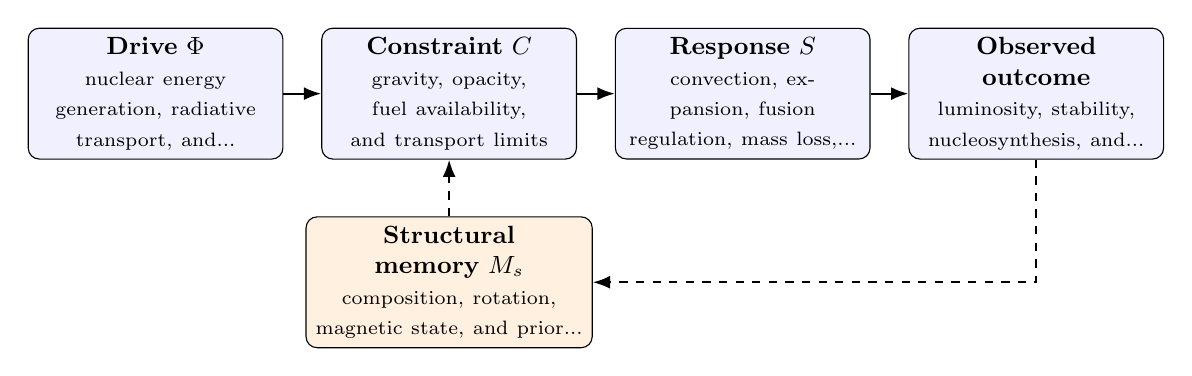
\begin{tikzpicture}[
    node distance=0.48cm,
    every node/.style={font=\small},
    box/.style={draw, rounded corners, align=center, minimum height=1.45cm, text width=3.0cm, fill=blue!6},
    memory/.style={draw, rounded corners, align=center, minimum height=1.25cm, text width=3.4cm, fill=orange!12},
    flow/.style={-{Latex[length=2.2mm]}, thick},
    feedback/.style={-{Latex[length=2.2mm]}, thick, dashed}
]
\node[box] (drive) {\textbf{Drive $\Phi$}\\\scriptsize nuclear energy generation, radiative transport, and...};
\node[box, right=of drive] (constraint) {\textbf{Constraint $C$}\\\scriptsize gravity, opacity, fuel availability, and transport limits};
\node[box, right=of constraint] (response) {\textbf{Response $S$}\\\scriptsize convection, expansion, fusion regulation, mass loss,...};
\node[box, right=of response] (outcome) {\textbf{Observed outcome}\\\scriptsize luminosity, stability, nucleosynthesis, and...};
\node[memory, below=0.72cm of constraint] (memory) {\textbf{Structural memory $M_s$}\\\scriptsize composition, rotation, magnetic state, and prior...};
\draw[flow] (drive) -- (constraint);
\draw[flow] (constraint) -- (response);
\draw[flow] (response) -- (outcome);
\draw[feedback] (outcome.south) |- (memory.east);
\draw[feedback] (memory.north) -- (constraint.south);
\end{tikzpicture}
\caption{Paper F-01 observable CDFD/AFL architecture for Stellar Evolution. Solid arrows give the proposed forward chain; dashed arrows make history-dependent feedback explicit.}
\label{fig:f01-architecture}
\end{figure}

\subsection{Minimal Coupled Model}

A paper-level model must separate throughput, constraint accumulation, response,
and history. One deliberately minimal form is
\begin{align}
Y(t) &= \frac{\Phi(t)S(t)}{\epsilon + C(t)}, \\
\frac{dC}{dt} &= \alpha \Phi(t) - \beta S(t)C(t) + \gamma \mathcal{L}C(t), \\
\frac{dM_s}{dt} &= \eta C(t) - \mu M_s(t), \\
\Psi_s(t) &= \frac{\widehat{\Phi}(t)}{\epsilon+\widehat{C}(t)}\,
             \widehat{S}(t)\,[1+\omega\widehat{M_s}(t)] .
\end{align}
Here $Y$ is the measured output, $\epsilon>0$ prevents a singular denominator,
$\mathcal{L}$ is a spatial or network coupling operator, and hats denote
explicitly normalized variables. The sign and magnitude of $\omega$ must be
estimated: memory can preserve useful organization or amplify damage. No fixed
threshold is universal before the variables, normalization, and observation
scale are declared.

For this paper, the hypothesized causal sequence is specific. A change in
nuclear energy generation, radiative transport, and mass flow arrives faster than convection, expansion, fusion regulation, mass loss, and mixing can compensate.
This raises or redistributes gravity, opacity, fuel availability, and transport limits. If the load persists,
the retained state encoded by composition, rotation, magnetic state, and prior burning stages changes the next response, so a later event of equal
magnitude can produce a different trajectory in luminosity, stability, nucleosynthesis, and evolutionary transition. The
scientific task is to estimate that sequence against the best ordinary model of
the domain, not merely to redescribe the outcome after it occurs.

\subsection{Cross-Scale Universality Without Mechanistic Erasure}

For the cosmic and subatomic systems family, the universal comparison must remain subordinate to conservation laws, relativity, quantum mechanics, and established astrophysical or plasma equations. CDFD is useful only if it compresses a regime transition or hysteresis question without pretending that biological adaptation and physical response are the same mechanism. \cite{Turing1952,Shannon1948,BakTangWiesenfeld1987}
The CDFD programme is cumulative: Part I supplies the flow--constraint
foundation \cite{MujjabiPartI2026}; Part II asks when maintained throughput
supports persistent organized states \cite{MujjabiPartII2026}; Part III
develops adaptive limitation and biological memory \cite{MujjabiPartIII2026};
and Part IV \cite{MujjabiPartIV2026} tests how much of that architecture
survives translation. The CDFD Runtime \cite{CDFDRuntime2026} supplies a
reproducible numerical stress surface, but it does not substitute for the
domain evidence named here.

The required scale declaration for this paper is seconds to billions of years; nuclei to stellar populations. At short
scales, the key question is whether the incoming drive is transmitted,
buffered, or diverted. At intermediate scales, response changes effective
capacity and network exposure. At long scales, retained structure can alter the
state space itself. A result is genuinely cross-scale only when the aggregation
rule is stated and the same conclusion is not an artifact of averaging.

\subsection{Evidence Ladder and Discriminating Tests}

\begin{table}[htbp]
\centering
\small
\caption{Evidence ladder for Paper F-01. Each rung can fail independently.}
\begin{tabularx}{\textwidth}{|p{0.17\textwidth}|X|X|}
\hline
\textbf{Test} & \textbf{Design} & \textbf{Discriminating result} \\
\hline
Proxy audit & Measure photometry, spectroscopy, asteroseismology, neutrinos, stellar populations, and models and preregister how each record maps to $\Phi$, $C$, $S$, $M_s$, and $Y$. & The mapping fails if proxies are non-identifiable, circular, or change meaning across cases. \\
\hline
Load ramp & Apply or observe a comparison across stars of matched mass but different composition or rotation while estimating the dominant constraint and response time. & A threshold claim requires a reproducible nonlinear change and uncertainty bounds, not a visually chosen breakpoint. \\
\hline
Recovery and memory & Match present load across units with different histories, then compare recovery paths. & The memory claim requires history-dependent divergence after current conditions are controlled. \\
\hline
Model comparison & Compare the baseline domain model with and without the CDFD/AFL state variables using held-out data. & The paper's stated falsifier is: the CDFD translation adds no testable prediction beyond stellar structure and evolution. \\
\hline
\end{tabularx}
\end{table}

The strongest practical design combines a prospective perturbation with a
recovery window. The load-ramp phase estimates where constraint begins to rise
faster than output. The recovery phase estimates $\beta$ and $\mu$, separating
fast relaxation from persistent memory. A topology or coupling intervention
then asks whether rerouting changes the cascade as predicted. Null results are
informative because they identify domains in which the universal notation adds
no measurable value.

\subsection{Research Programme and Boundary Conditions}

The immediate research programme has four steps. First, construct a documented
dataset from photometry, spectroscopy, asteroseismology, neutrinos, stellar populations, and models and retain raw units before normalization.
Second, fit a baseline domain model and report its calibration and out-of-sample
error. Third, add the smallest identifiable CDFD/AFL state extension and test
whether it improves prediction of luminosity, stability, nucleosynthesis, and evolutionary transition. Fourth, repeat the
analysis across the declared scale range and publish negative cases as part of
the universality audit.

Three boundaries are non-negotiable. Correlation between flow and failure does
not identify a constraint mechanism. A fitted memory term does not prove that
the stored state has the same material meaning in another domain. Finally, a
runtime cascade is evidence about the implementation, not evidence that the
real system follows it. The paper becomes stronger when it can say precisely
where the translation stops.


% END PART IV MAJOR UNIVERSAL UPGRADE

\section{Conclusion}
By mapping stellar nucleosynthesis and hydrostatic equilibrium into the CDFD ontology, we uncover a unifying topological continuity. A star operates under a comparable normalized flow--constraint architecture of flow limitation, constraint resistance, and memory accumulation that govern pre-biotic chemical networks and biological metabolism. The Main Sequence is a candidate normalized operating regime.

\section*{Conflict of Interest} The author declares no conflict of interest.
\section*{Data Availability}
Part-specific runtime diagnostics are under each Part's \path{outputs/} directory.

Release-wide code: \path{Part_E_Synthesis/supplementary/}.

Generated summaries: \path{Part_E_Synthesis/outputs/}.

Figures: \path{Part_E_Synthesis/figures/}.


\section{Reference Layer}
\bibliographystyle{plain}
\bibliography{universal_afl_references}
\end{document}
